\documentclass{beamer}

\usepackage[utf8]{inputenc}
\usepackage[english]{babel}
\usepackage[T1]{fontenc}
\usepackage{lmodern}
\usepackage{graphicx}
\usepackage{commath}
\usepackage{amsmath,amssymb,amsthm}
\usepackage[lined]{algorithm2e}
\usetheme{Singapore}
\newlength{\mylen}
\begin{document}

\title{Integrate lexical constraints and background knowledge to $K$-Means with Deep Learning}
\author{Maxence Grand \and \\                                                   
        Supervised by : \'Eric Gaussier \and Thibaut Thonet \and Marc Tommasi \and Aur\'elien Bellet \and Maziar Moradi Fard} 
\institute{Laboratoire d'Informatique de Grenoble, Team AMA}
\date{\today}

\maketitle

\section{Introduction}

\begin{frame}
\frametitle{Lexical Constraints}

\end{frame}

\begin{frame}
\frametitle{Background Knowledge}
\begin{itemize}
\item \textbf{Must-link} constraint $ML$ : $(X, X') \in ML \implies $ X and X' are in the
  same cluster.
\item \textbf{Cannot-link} constraint $CL$ : $(X, X') \in CL \implies $ X and X' are in
  different cluster.
\end{itemize}
\end{frame}

\section{Related Work}

\begin{frame}
\frametitle{$K$-Means}
Given a corpus C, where each document X is a 
d-dimensional real vector, k-means clustering aims to partition the n 
documents into K $S_k$ clusters represented by centroids 
R = {$r_1, r_2, ..., r_K$}. :
Formally, the objective is to minimize :
$$
\sum_{k =1 }^K \sum_{X \in S_k} ||X - r_k||_2^2
$$
\end{frame}

\begin{frame}
  \frametitle{Auto-Encoder}
  \begin{columns}[T] % align columns
    \setlength{\mylen}{0.4\textwidth}
    \begin{column}{\mylen}
      \begin{figure}[!h]
        \centering
        \fbox{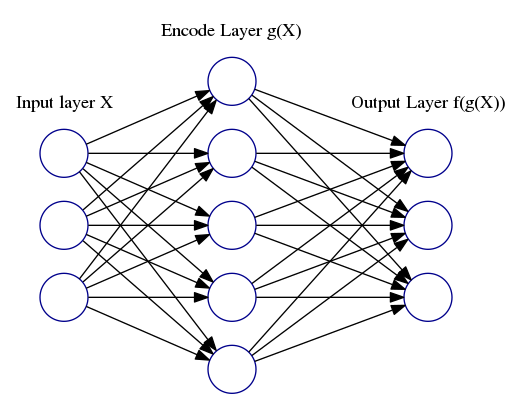
\includegraphics[scale=0.28]{autoencoder.png}}
        \caption{Auto-Encoder}
        \label{fig:AE}
      \end{figure}
    \end{column}%
    \hfill%
    \begin{column}{\dimexpr\textwidth-\mylen}
      \pause
      \begin{itemize}
        \setlength\itemsep{2em}
      \item Encode Function $g(X; \theta)$ \pause
      \item Decode Function $f(g(X; \theta)$ \pause
      \item $L_{rec}(X, \theta) = || X - f(g(X, \theta)) ||_2^2$
      \end{itemize}
    \end{column}%
  \end{columns}
\end{frame}

\begin{frame}
  \frametitle{Background Knowledge - COP$K$-Means}
  \begin{columns}[T] % align columns
    \setlength{\mylen}{0.5\textwidth}
    \begin{column}{\mylen}
      \scalebox{.7}{                        %new code
        \begin{algorithm}[H]
          \SetKwInOut{Input}{input}
          \SetKwInOut{Output}{output}
          \Input{Corpus C, must-link constraints $ML \subseteq C x C$,
            cannot-link constraints $CL \subseteq C x C$}
          \Output{Clusters $S_1, S_2, ..., S_k$}
          Let $S_1, S_2 , ..., S_k$ be the initial clusters\\
          \Repeat{Convergence}{
            \ForEach{$X_i \in C$}{
              Assign $X_i$ to closest $S_j$ such that Violate-Constraints($X_i, C_j, CL,
              ML$) is false.\\
              \If{No such clusters exists}{
                return \{\}\\
              }
            }
            \ForEach{Clusters $S_i$}{
              Update centroids.\\
            }
          }
          \Return{$S_1, S_2, ..., S_k$}
          \caption{\label{algo:cop}COP-Kmeans}
        \end{algorithm}  
      }
    \end{column}%
    \hfill%
    \begin{column}{\dimexpr\textwidth-\mylen}
      \scalebox{.7}{                        %new code
        \begin{algorithm}[H]
          \SetKwInOut{Input}{input}
          \SetKwInOut{Output}{output}
          \Input{Ducument X, Clusters S, must-link constraints $ML \subseteq C x C$,
            cannot-link constraints $CL \subseteq C x C$}
          \Output{True if constraints are violate, False otherwise}
          \ForEach{($X, X' \in ML$)}{
            \If{$X' \in S$}{
              \Return{True}
            }
          }
          \ForEach{($X, X' \in CL$)}{
            \If{$X' \in S$}{
              \Return{True}
            }
          }
          \Return{False}
          \caption{\label{algo:vio}Violate-Constraints}
        \end{algorithm}

      } 
    \end{column}%
  \end{columns}
\end{frame}

\begin{frame}
\frametitle{Background Knowledge - NNClustering}
\begin{equation*}
  P = f(x_p), ~ Q = f(x_q)
\end{equation*}

\begin{equation*}
  KL(P||Q) = \sum_i^k P_ilog\frac{P_i}{Q_i}
\end{equation*}

\begin{equation*}
  I_s = \left\{
\begin{array}{ll}
  1 & \mbox{if $x_p$ and $x_q$ is a similar pair}\\
  0 & \mbox{Otherwise.}
\end{array}
\right.
\end{equation*}
%
\begin{equation*}
  I_{ds} = \left\{
\begin{array}{ll}
  1 & \mbox{if $x_p$ and $x_q$ is a dissimilar pair}\\
  0 & \mbox{Otherwise.}
\end{array}
\right.
\end{equation*}
\begin{equation*}
  Loss(P || Q) = I_s(x_p, x_q)KL(P || Q) + I_{ds}(x_p, x_q)max(0,
  \eta-KL(P||Q))
\end{equation*}
\begin{equation*}
  L(P,Q) = Loss(P || Q) + Loss(Q || P)
\end{equation*}
\end{frame}


\begin{frame}
\frametitle{Deep Clustering - General Form}
\begin{itemize}
\item \textbf{Non-Clustering loss} : $L_{NonClust}(C;\theta)$
\item \textbf{Clustering loss} : $L_{Clust}(C;\theta)$
\end{itemize}
\pause
The loss function takes the form :
\begin{equation*}
L(X;\theta) = \lambda L_{NonClust}(C;\theta) + (1-\lambda)L_{Clust}(C; \theta)
\end{equation*}
Where $\lambda \in [0 ; 1]$

\end{frame}
\begin{frame}
  \frametitle{Deep $K$-Means }
\begin{equation*}
L(C ,\beta;\theta,R) = L_{NonClust}(C;\theta,R ) + \lambda L_{Clust}(C,\beta;\theta,R)
\end{equation*}
\begin{equation*}
L_{NonClust}(C;\theta,R ) = \sum_{X \in C} ||X - f(g(X;\theta))||_2^2
\end{equation*}
\begin{equation*}
  L_{Clust}(C,\beta;\theta,R) = F(g(X),c(g(X, \theta); R))
\end{equation*}
\end{frame}

\begin{frame}
  \frametitle{Deep $K$-Means }
\begin{equation*}
L_{Clust} = \sum_{k=1}^K F(g(X; \theta), r_k) G_{k, F}(g(X; \theta), \beta; R)
\end{equation*}
\begin{equation*}
G_{k, F}(g(X; \theta), \beta; R) = \frac{e^{-\beta F(g(X, \theta),r_k)}}
{\sum_{k' = 1}^K e^{-\beta F(g(X, \theta),r_k')}}
\end{equation*}
\end{frame}
\section{Proposed Method}

\begin{frame}
\frametitle{The Idea}
Learn a latent space taking into account lexical constraints and
background knowledge.
\pause
\begin{equation*}\label{eq:h}
  h_X = g(X,\theta)
\end{equation*}
\end{frame}

\begin{frame}
\frametitle{Lexical Constraints}
\begin{equation*}
KW = \begin{pmatrix} kw_1 & kw_2 & ... & kw_{k-1} & kw_{k}
\end {pmatrix}
\end{equation*}
\pause
\begin{equation*}
\forall_{i=1,2,..,n}X_i' = \left\{
\begin{array}{ll}
  X_i & \mbox{if } i \in KW \\
  0 & \mbox{Otherwise.}
\end{array}
\right.
\end{equation*}
\pause
\begin{equation*}\label{eq:omega1}
  \omega_{KW} = \sum_{X \in C} || h_{X} - h_{X'}||_2^2
\end{equation*}
\end{frame}

\begin{frame}
\frametitle{Background Knowledge}
\pause
\begin{itemize}
\item Must-Link : $$\omega_{ML} = \sum_{\forall{(X_i,X_j)\in ML}} || h_{X_i} - h_{X_j} ||_2^2$$ \pause
\item Cannot-Link : $$\omega_{CL} = \sum_{\forall{(X_i,X_j)\in CL}} max(0,
  \eta - || h_{X_i} - h_{X_j} ||_2^2)$$
\end{itemize}
\end{frame}

\begin{frame}
\frametitle{Non Clustering Loss}
\begin{equation*}\label{eq:Sparse}
  \Omega(C) = \alpha_0\omega_{KW} + \alpha_1\omega_{CL} + \alpha_2\omega_{ML}  
\end{equation*}
\pause
\begin{equation*}
  L_{rec}(C, \theta) = \sum_{X \in C}(||X - f(g(X, \theta))||_2^2
\end{equation*}
\pause
\begin{equation*}
  L_{NonClust}(C,KW; \theta) = L_{rec}(C, \theta) + \Omega(C)  
\end{equation*}

\end{frame}

\begin{frame}
\frametitle{Deep $K$-Means}
$$R = \begin{pmatrix} r_1 & r_2 & ... & r_K\end{pmatrix}$$
\pause
\begin{equation*}
  L_{Clust}(C, K; \theta) = \sum_{k=1}^K F(h_X, r_k) G_{k, F}(h_X, \beta; R) 
\end{equation*}
\pause
\begin{equation*}
  Min~L(KW, C, K; \theta) = L_{NonClust}(C, KW; \theta) + \lambda.L_{clust}(C,K;\theta)
\end{equation*}
with $\lambda \geq 0$
\end{frame}

\section{Experiment}

\begin{frame}
\frametitle{Data}
\end{frame}

\begin{frame}
\frametitle{Lexical Constraints}
\end{frame}

\begin{frame}
\frametitle{Architecture}
\end{frame}

\begin{frame}
\frametitle{Hyperparameters}
\end{frame}

\begin{frame}
\frametitle{Results}
\end{frame}

\section{Futur Work}

\begin{frame}
\frametitle{Pairwise Constraints}
\end{frame}

\begin{frame}
\frametitle{More Baseline Algorithm}
\end{frame}

\section{Conclusion}

\begin{frame}
\frametitle{Conclusion}
\end{frame}

\begin{frame}
Any Question ?
\end{frame}

\section*{Conclusion}

\begin{frame}
\frametitle{Additionnal}
\end{frame}
\end{document}
